\documentclass{standalone}
\begin{document}
\section{Chapter 2 Human Factors}
\begin{itemize}
	\item The goal is to \textbf{stimulate all perception channels in such a way that the user feels completely immersed in the virtual environment and accepts it as real.}
	\item we are forced by our senses to perceive every environment in the sameway, nomatter wheter this environment is real or virtual
	\item visual(80\%), acoustic(10\%), thermal(2\%), haptic(5\%) and olfactory(3\%) perception($80\%$ of the overall information is perceived via the visual channel)
	\item Human Perception
	\begin{itemize}
		\item Perception
		\begin{itemize}
			\item Sensous physiology (sensory): the perception of stimuli, performed by sensory cells or by sensory organs.
			\item Psychology : Process of sensuous perception of an object \textbf{without any conscious identification} of the perceived object.
		\end{itemize}
		\item Cognition
		\begin{itemize}
			\item Psychology : Collective name for all processes or structures that are involved in the \textbf{cognition} process. e.g. imagination, estimation, memory, remembrance, learning. etc 
			\item i.e. interpretation of perception
		\end{itemize}
	\end{itemize}
	\item Four elementary attributes of stimulus
	\begin{itemize}
		\item modality: quality of a stimulus(the \textbf{type of physical energy} that is responsible for the stimulus)
		\item intensity: The \textbf{strength} of a stimulus defines the intensity of a sensation(below a specific threshold, the stimulus is not detected
		\item duration: relationship between the intensity of the stimulus and the \textbf{duration} of the sensation defines the perceived intensity (Note: adaptation - stimulus persist for long time $\rightarrow$ intensity decrease)
		\item location: The ability to locate the \textbf{position} of a stimulus and the ability to distinguish between two spatially close stimuli are important measures of the awareness of the spatial distribution of a sensory experience
	\end{itemize}
	\item action potential: Only if the intensity is larger than a particular \textbf{threshold}, an electrical discharge is generated by the responsible receptors
	\item only the sensory part (sensous physiology of perception) of the cognition process can be addressed by devices of the virtual environment. (Figure)
\end{itemize}
\begin{figure}[H]
\centering
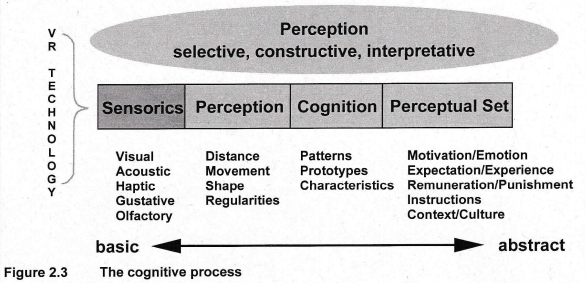
\includegraphics[width = 0.7\linewidth]{Figures/2_3.png}
\end{figure}
\subsection{The Human Eye}
\subsubsection{Viewing Angle}
\begin{itemize}
	\item Field of view characterized by: optical setup of the eye / the position of the eye in the face
	\item although field of view is very large perception of sharp images only possible in much smaller area ($2 \sim 3\deg$)
	\item viewing cones of both eyes overlap in a range of approximately 120 degrees
	\item Four opening angles of the field of view
\begin{table}[H]
\centering
\begin{tabular}{|l|c|c|r|}
\hline
 nasal & temporal & superior & inferior \\ \hline
60 deg & 100 deg & 60 deg & 70 deg \\ \hline
\end{tabular}
\end{table}
	\item resolution: in the distance of 5 m, resolve object 1.5 mm away from each other. ($\approx 8400 \times 5400 px$)
	\item Note 
		\begin{itemize} 
			\item FOV w/o turning head $= 155\deg$ (horizontal), $113\deg$ (vertical) 
			\item FOV w turning head $= 300\deg$ (horizontal), $283\deg$ (vertical) 
		\end{itemize}
\end{itemize}
\subsubsection{Temporal Resolution}
\begin{itemize}
	\item pupil can adapt to changing light conditions with a maximum frequency of 4 Hz	
	\item flicker consolidation frequency: frequency without noticing any flickering
	\item perception of flickering not only depends on brightness but also the size of field of view and the location of light source in the FOV
\end{itemize}

\begin{figure}[H]
	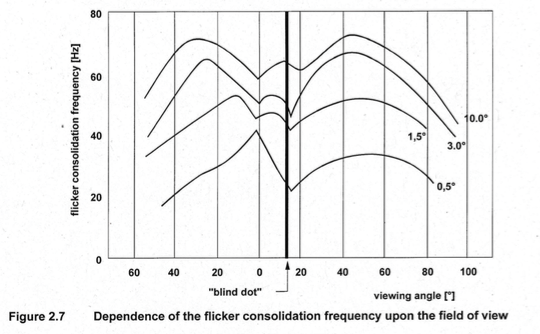
\includegraphics[width=\linewidth]{2_7}
\end{figure}

\subsubsection{Accommodation and Convergence}
\begin{itemize}
	\item eye focuses onto shortest possible distance until object is visible: needs edges, patterns or contours to focus: In complete darkness, the eye cannot focus anymore
	\item results in near sightedness when looking through a optical device (e.g. Head Mounted Display)
	\item convergence: depth estimation up to 10 meters is made with stereoscopic vision ($\epsilon$ is convergence angle) $\tan \frac{\epsilon}{2} = \frac{a}{2} \frac{1}{e}$
	
	\begin{figure}[H]
		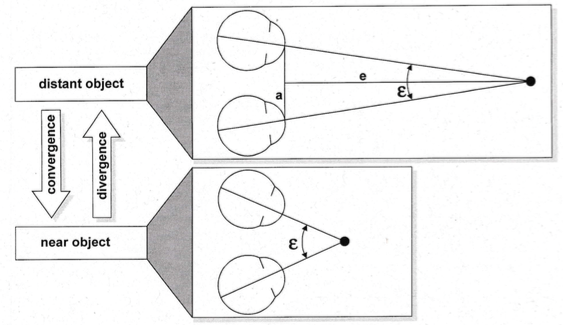
\includegraphics[width=\linewidth]{2_8}
	\end{figure}
	
	\item accommodation: optical adaptation of the eye to different distances by changing the refraction of the lens (by muscle: straining muscle $\rightarrow$ thicker lens $\rightarrow$ near object)
	\item Note: when using a stereoscopic projection (displaying two images for sense of 3D), only convergence causes the stereoscopic effect. (accommodation stays constant: distance to display)
\end{itemize}


\setcounter{subsubsection}{4}
\subsubsection{B/W Perception, Color Perception}
\begin{itemize}
	\item some terminologies...
		\begin{itemize}
			\item brightness: surface emits more or less light (subjective: cannot be measured)
			\item luminance: measure of the energy flow. (measurement)
			\item color: more details $\downarrow$ (subjective)
			\item color temperature: based on Planck's black light source - color of emitted light $\propto$ temperature (measurement)
		\end{itemize}
	\item light models: wave-model is more sufficient (vs photon model) - regarding the light as a electromagnetic radiation with a wavelength between 380 nm and 780 nm
	\item color perception is done by a single eye
	\item color is perceived using special receptors on the retina
		\begin{itemize}
			\item \textbf{sticks} : only measure the intensity of the incoming light(Black and White). used at night but easily saturated. (more sensitive than uvulas)
			\item \textbf{uvulas} : used in daylight(light at night are not sufficient to work for uvulas), different uvulas for each color : (blue-sensitive uvulas 4 \% at 430 nm , green-sensitive uvulas 32 \% at 530 nm, red sensitive uvulas 64 \% at 560 nm) 
			\item Note: red sensitive uvulas are the most but human eye is most sensitive in green.
			\item 95 \% are sticks and 5 \% are color sensitive uvulas
		\end{itemize}
	\item color processing + B/W
		\begin{itemize}
			\item 2 channel: (red - green), (yellow - blue). 
			\item non-colored brightness: red + green + blue (brightness from uvulas)
			\item brightness from stick
			\item processed in retina 
			\item 
				\begin{figure}[H]
				\centering
				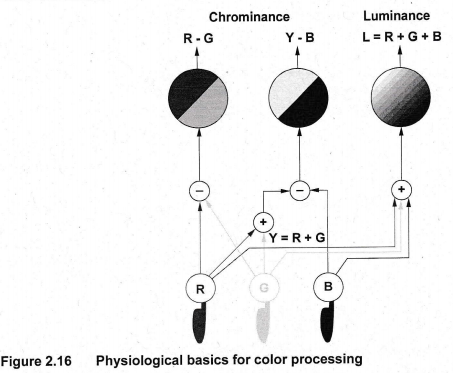
\includegraphics[width = 0.5\linewidth]{Figures/2_16.png}
				\end{figure}			
			\item daylight: different kind of uvulas capture the basic colors red, green and blue while the sticks only measure brightness (if sticks are saturated $\rightarrow$ brightness from stick is useless)
			\item darkness: uvulas do not provide any color information, but only black(no info.), small amount of light is sufficient to activate the sticks. $\rightarrow$ only black and white image
		\end{itemize}
\item Note: hue, saturation, brightness imitate the human color perception
\item contrast amplification: in order to increase the perceived sharpness of the image
\item chromostereopsis: focal length depends on the color. If more colors exist at the same distance, the eye can only focus on one of them. (e.g. if red, blue exist, the eye will focus on the red field due to the larger amount of red sensitive receptors) Chromostereopsis is used in displaying topographical maps. (induces fatigue)
\end{itemize}

\subsubsection*{Color Models}
\begin{itemize}
		\item color models: classification and measurement of colors
		\item CIE color model(Commission Internationale del'Eclairage):
			\begin{itemize} 
				\item based on the typical sensitivity of the different uvulas (perception oriented color model)
				\item for selected color's $F(\lambda)$:
					\begin{align}
						X &= \int_{380nm}^{780nm} F(\lambda) \cdot \bar{x}(\lambda) d\lambda \text{blue}\\
						Y &= \int_{380nm}^{780nm} F(\lambda) \cdot \bar{y}(\lambda) d\lambda \text{green}\\
						Z &= \int_{380nm}^{780nm} F(\lambda) \cdot \bar{z}(\lambda) d\lambda \text{red}
					\end{align}
				\item Note: human eye - many red sensitive uvulas but only in a small bandwidth $\rightarrow$ more sensitive to green. 
			\end{itemize}
		\item YUV color model: Takes account the high green sensitivity into, while sensitivity to red and blue is significantly lower (perception oriented color model)
		\begin{align}
			C_b &= B - Y \quad \text{color difference signal 1}\\
			C_r &= R - Y \quad \text{color difference signal 2}\\
			Y & \quad brightness (luminance)
		\end{align}
		\item \textbf{RGB color model}
			\begin{itemize} 
				\item does not take the physiology of the human eye into account(technical color model)
				\item basic colors (red, green and blue) are scaled to 1 and define a coordinate system
				\item for object which emits light
				\item additive model: $F = r \cdot R + g \cdot G + b \cdot B$
				\item color cube:
					\begin{figure}[H]
						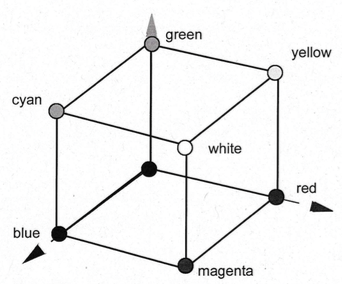
\includegraphics[width=\linewidth]{2_24.png}
					\end{figure}
			\end{itemize}
		\item \textbf{CMY color model}
			\begin{itemize}
			 	\item used by objects that do not emit light themselves: reflected light = color (e.g. color used by printers)
			 	\item absorption or subtractive model.
			 	\item color cube: magenta, yellow, cyan is on the axis, white is on the origin.
			 	\item $[R, G, B] = [1, 1, 1] - [C, M, Y]$
			 \end{itemize}
		\item \textbf{HSV color model(also HSB)}: 
			\begin{itemize} 
				\item Defined by hue, saturation, value. In this color model, colors are arranged in a circle around the vertical axis
				\item hue: $0\deg \rightarrow$ red, $120\deg \rightarrow$ green, $240\deg \rightarrow$ blue
				\item saturation: 0 $\sim$ 255
				\item intensity: 0 $\sim$ 255
			\end{itemize}
\end{itemize}
\subsubsection{Three-dimensional Viewing}
\subsubsection*{Spatial Viewing}
\begin{itemize}
\item spatial viewing can be performed with only one eye and thus is also called monocular viewing(only psychological aspects are considered)
	\begin{itemize}
		\item Size of the Image on the Retina: If the real size is known, the brain compares the perceived size with the real size stored in the brain and calculates information of the position and the distance of the object
		\item Resoultion of the Perceived Image: Objects with blurred surface appear far away
		\item Overlap: If one object is in front of the other it has to be closer to the spectator than the object
		\item perspective: Far objects appear smaller than close ones
		\item shaded objects and shadows: I the light source is know, the object that causes the shadow appears closer to the light source
		\item textures: A spatial effect also appears when mapping textures perspectively onto an object. Wrong selection of textures could completely camouflage the geometry or pretend a wrong geometry
		\item motion parallax: the farther away an object is, the slower it moves on the retina when moving relatively to the user
	\end{itemize}
	\item Perception Rules Depending on geometry
	\begin{itemize}
		\item Rules of proximity: Spatially or temporally neighboring elements are perceived to belong together and to be part of the same element
		\begin{figure}[H]
			\centering
			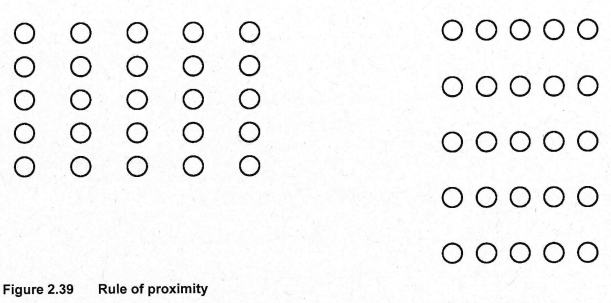
\includegraphics[width = 0.5\linewidth]{Figures/2_39.png}
		\end{figure}
		\item rule of similarity/rule of identity: Similar or identical objects appear coherently 
		\begin{figure}[H]
			\centering
			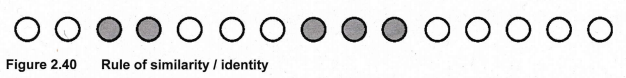
\includegraphics[width = 0.5\linewidth]{Figures/2_40.png}
		\end{figure}
		\item identity versus proximity: effects can be amplified or reduced
		\begin{figure}[H]
			\centering
			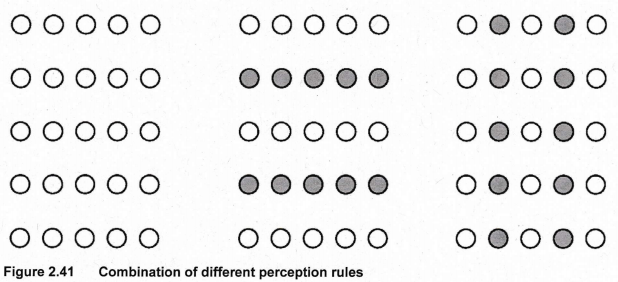
\includegraphics[width = 0.5\linewidth]{Figures/2_41.png}
		\end{figure}
		\item rule of harmonic continuation: elements that are spatially or temporally arranged in a simple harmonic or well defined order appear coherently and thus belong to the same geometric figure
		\begin{figure}[H]
			\centering
			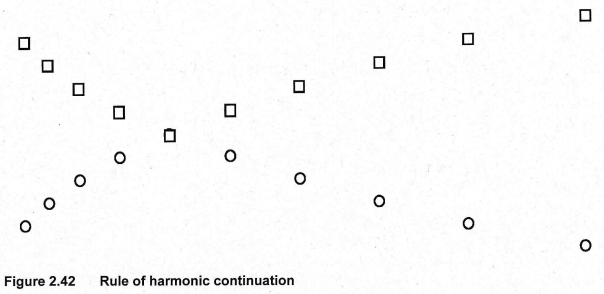
\includegraphics[width = 0.5\linewidth]{Figures/2_42.png}
		\end{figure}
		\item rule of closed lines: Contours, which are not completely closed, will be automatically closed during the perception process
			\begin{figure}[H]
				\centering
				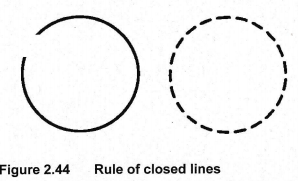
\includegraphics[width = 0.5\linewidth]{Figures/2_44.png}
				\end{figure}
		\item rule of symmetry: if none of the mentioned rules could be applied, the space between symmetric contours shapes a figure, rather than the space between asymmetric contours
			\begin{figure}[H]
				\centering
				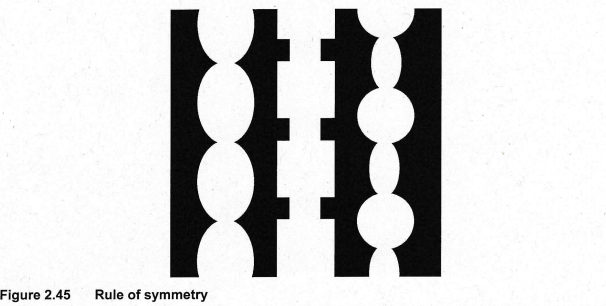
\includegraphics[width = 0.5\linewidth]{Figures/2_45.png}
			\end{figure}
		\item the principle of harmonic shape: The structure will be perceived, that has as many simple figures as possible
			\begin{figure}[H]
			\centering
			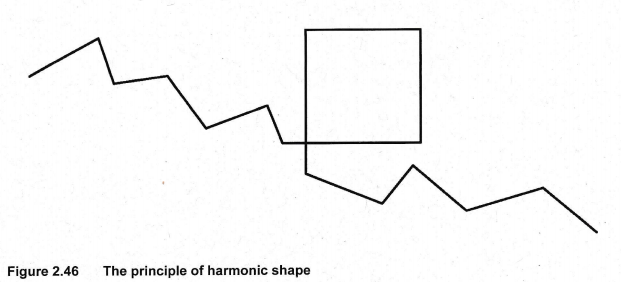
\includegraphics[width = 0.5\linewidth]{Figures/2_46.png}
			\end{figure}
		\item contours: there's certain force to see contours.
			\begin{itemize}
				\item but this kind of perception only works if the user has seen the shape(e.g. triangle in the following figure) before.
				\item known patterns paly an important role.
			\end{itemize}
			\begin{figure}[H]
			\centering
			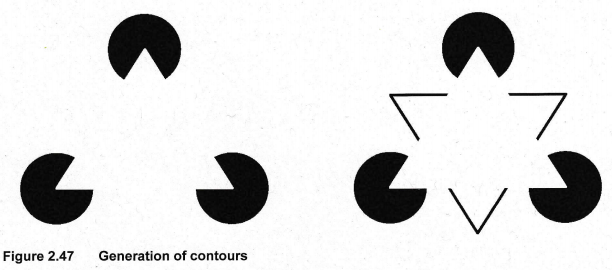
\includegraphics[width = 0.7\linewidth]{Figures/2_47.png}
			\end{figure}
	\end{itemize}
\end{itemize}
\subsubsection*{Allocation Problems - illusions}
\begin{itemize}
	\item The reason for allocation problem is the fact that the interpretation of the perceived impression is done in different parts of the brain (e.g. color - right brain, reading - left brain : Figure 2.54)
	\item wrong perspective: in reality, perspective point is only one (Figure 2.48)
	\item brightness of objects given context: absolute brightness cannot be percieved (Figure 2.49)
	\item comparison with known patterns: if the objects seems to be compatible with stored pattern (Figure 2.50)
	\item peripheral drift illusion (Figure 2.51, 2.52)
		\begin{itemize}
			\item static images seem to move when viewing at different areas of the image
			\item depends on difference in brightness : from black to dark gray / white to light gray
		\end{itemize}
	\item Hermann grid
		\begin{itemize}
			\item due to the contrast amplification by neurons.
			\item white or gray grid on a black background. 
			\item width of the white lines corresponds to the diameter of the receptive fields on the retina(contrast amplification by ON-center neurons, OFF-center neurons)
			\item seems like gray dots are on the cross-sections
			\item white line is perceived to be very light, but crossing is perceived to be less light.
		\end{itemize} 
		\begin{figure}[H]
			\centering
			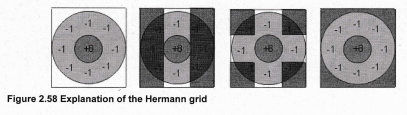
\includegraphics[width = 0.7\linewidth]{Figures/2_58.png}
		\end{figure}
		\item scintillating grid
			\begin{itemize} 
				\item consists of a herman grid with gray lines on a black background, with white dots on the crossing(effect: outside the zone of interest, black dots appear instead of original white dots)
				\item due to unconscious moves of eye balls (but since user cannot focus on the black dots it only appears temporarily)
				\item unlike the Hermann grid, this effect to intensive, and cannot be explained by a simple contrast phenomenon.
			\end{itemize}
		\begin{figure}[H]
			\centering
			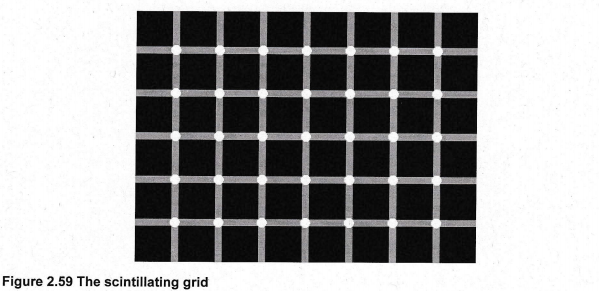
\includegraphics[width = 0.7\linewidth]{Figures/2_59.png}
		\end{figure}
		\item barber's pole effect: rotating cylinder with spiral(motion is always in direction of the aperture's longest edge)
\end{itemize}
\subsubsection*{Stereoscopic viewing}
\begin{itemize}
	\item \textbf{physiological aspects!}
	\item In order to focus both eyes on the object, they are directed onto the object. This will result in a convergence angle between the optical axes of both eyes	
	\item by disparity (horizontal parallex), brain generate 3D image
	\item The point is projected on non-corresponding areas on the retina on both eyes. This gives a spacial impression
	\item only works for $<$ 10 m 
\end{itemize}
\subsubsection{Conflicts between Virtual Reality and the Physiological and Psychological Visual Perception}
\begin{itemize}
	\item Since all virtual objects are visible on the projection plane (2D screen), the human eye does not have to perform an accommodation(physiological) anymore, but only focuses on the given distance between the user and the projection plane
	\item 3D impression still possible but eyes are easily fatigued
	\item psychological aspects are also not fulfilled (e.g. perception of size, resolution etc.)
	\item in VR physiologic and psychology perceptions are not combined anymore. $\rightarrow$ rapid fatigue
\end{itemize}

\subsection{The Human Ear}
\begin{itemize}
	\item Functionality of hearing
		\begin{itemize}
			\item identification of objects (sound signal and sources)
			\item spatial orientation (location of sound source)
			\item protection / warning
			\item social contact (communication)
			\item psychological factors
		\end{itemize}
	\item properties: sound signal and source / location / sensitivity and loudness
	\item When simulating objects in virtual environments, the acoustical sensation is very important
	\item sound $\rightarrow$ transmission $\xrightarrow[\text{signal}]{}$ sense cell $\xrightarrow[\text{electric pulse}]{}$ brain 
\end{itemize}

\setcounter{subsubsection}{1}
\subsubsection{Spatial Hearing}
Spatial hearing desribes the accoustical determination of a sound source's position in a room. Two principles:
\begin{itemize}
	\item monaural hearing (one ear)
	\begin{itemize}
		\item Using one ear only: very rough localization($\pm 20 \deg$ deviation from correct localization) : does not play important role
	\end{itemize}
	\item binaural hearing (two ears)
	\begin{itemize}
		\item difference in intensity (by acoustical shadow): only possible if wavelength of the sound is small compared to the size of the head 
		\item difference in runtime: brain capable of detect runtime differences of approximately 30 us
		\item resolution: can calculate by the following $\rightarrow$ $3\deg$ (should be large than $3\deg$)
			\begin{align}
				\Delta x &= d sin \alpha \\
				\Delta t &= \frac{\Delta x}{c} = \frac{d}{c} sin \alpha \quad c = 340m/s
			\end{align}
	\end{itemize}
	\begin{figure}[H]
			\centering
		\begin{subfigure}[b]{0.45\textwidth}
			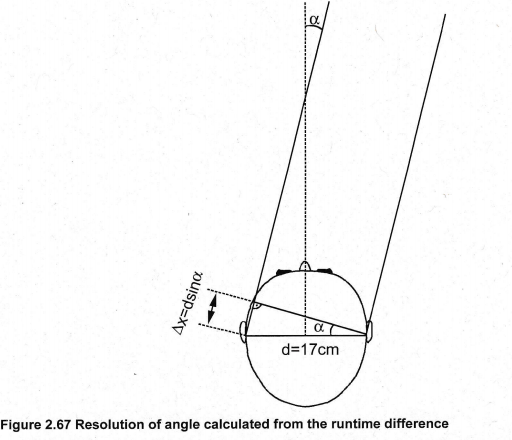
\includegraphics[width = 0.7\linewidth]{Figures/2_67.png}
		\end{subfigure}
		\begin{subfigure}[b]{0.45\textwidth}
			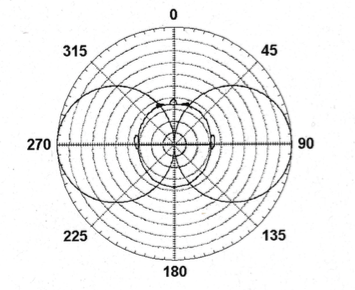
\includegraphics[width = 0.7\linewidth]{Figures/2_68.png}
		\end{subfigure}
		\end{figure}
\end{itemize}

\setcounter{subsubsection}{3}
\subsubsection{Allocation Problems of the Ear}

\begin{itemize}
	\item does not have many allocation problems. 
	\item Shephard effect: simulates increasing melody to the user although the pitch stays constant all the time
\end{itemize}

\subsection{The Haptic Channel}
\subsubsection{The Human Information Flow}
\begin{itemize}
	\item the entirety of all perceptions through the sense of touch
	\item about 80 \% of all information is perceived by the visual sense, other 15 \% by the auditory sense. The remaining 5 \% are for the haptic and olfactory sense. 
	\item but still important for immersion
	\item human information flow: environment $\rightarrow$ human $\rightarrow$ environment
		\begin{itemize}
			\item human perception: $10^9$ bit/s from env.
			\item only 10 $\sim$ 100 bit/s is perceived consciously. 
			\item human emission: $10^7$ bit/s (via speech, gesture ...)
		\end{itemize}
\end{itemize}
\subsubsection{The Haptic Perception}
\begin{itemize}
	\item The haptic takes place all over the body, thus it is impossible to generate a complete simulation in the haptic field: The human hand is the most relevant element in the field of haptics
	\item well known input device: mouse and keyboard provide haptic feedback addition to acoustic feedback.
	\item required for teleoperation
	\item Using the had to perform a manipulation
	\begin{itemize}
		\item Contact Phase: Describes the first contact of the fingers with an object(felt 200 ms after contact)
		\item Grasping Phase: has the largest flexibility and interactability
		- Grasping for increased power / Grasping with increased dexterity
		\item Touching Phase: For characterizing the properties of objects, different hand-object interactions are needed
	\end{itemize}
	\item Grasping can be seperated with thwo fields
	\begin{itemize}
		\item grasping with increased power
		\item grasping with increased dexterity
	\end{itemize}
	\item Haptic desribes the influence of foces of any kind onto the human body(tactile propriorceptive, kinesthetic)
	\begin{itemize}
		\item tactile: using perception cells in the skin(pressure, temperature, vibration)
		\item propriorceptive: Influence of force caused by the weight of the object onto the sensors in the musculature
		\item kinesthetic sensation is the perception of acceleration forces onto the body 
	\end{itemize}
	\item some haptic information can be directly processed in the skin nearby the sensor(reflex reaction allows much faster reaction)
\end{itemize}
\subsubsection*{Basics on the Physiology of the Senses in the Skin}
\begin{itemize}
	\item Skin registers pressure, touch, vibration (=sense of touch), temperature and pain. This surface sensibility (together with the depth sensibility (muscle, joint and string receptors)) is also called somatovisceral sensibility
	\begin{figure}[H]
			\centering
			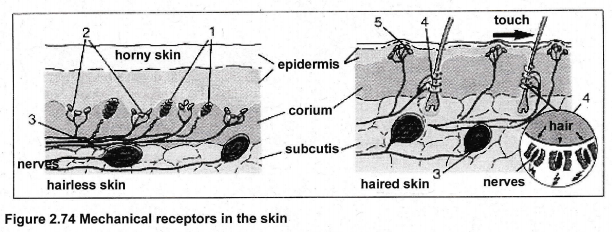
\includegraphics[width = 0.7\linewidth]{Figures/2_74.png}
	\end{figure}
	\begin{itemize}
		\item Meissner corpuscles(Fig.2.74->1): rapidly adapting receptors, provide information about the movement across the skin and thus velocity
		\item Merkel's Disks: slowly adapting receptors, react on pressure stimuli and provide information about vibrations
		\item Pacininan corpuscles(Fig.2.74->3): rapidly adapting receptors, sense acceleration as well as light touch and vibrations
		\item Raffini corpuscles detect pressure and skin shear as well as thermal changes
		\item Hair-root plexus(Fig.2.74->4) also called follicle, principle mechanoreceptor detects any movement on the skin surface
		\item Meissner cells(Fig.2.74->1) and hair receptors(Fig.2.74->4): detect the touch.(Not the intensity is important(bending of the hair) but the speed by the sensation changes.
		\item Pacini cells(Fig.2.74->3) specialized to detect vibrations
	\end{itemize}
	\item receptors can be divided into slowly adapting and rapdily apdapting mechanoreceptors
	\begin{itemize}
		\item rapidly adapting receptors respond to onset and often also termination but not throughout during stimulus-> sensorial adaptation
	\end{itemize}
	\item receptors can be classified by spatial resolution and temporal resolution
	\begin{itemize}
		\item intensity receptors: P-receptors
		\item speed receptors: D-receptors
		\item PD receptors are a mixture, which measure for example the position of the joints
	\end{itemize}
	\item Thermo receptors exist for a temperature range below 36 degrees(cold receptors) and for a temperature range above 36 degrees(heat receptors)
\end{itemize}
	\begin{figure}[H]
			\centering
			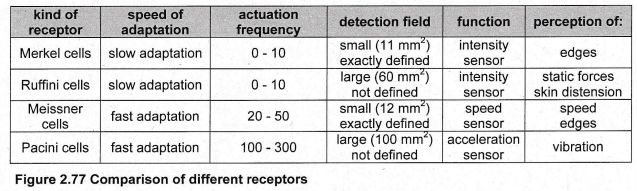
\includegraphics[width = 0.7\linewidth]{Figures/2_77.png}
	\end{figure}
\subsection{The collaboration of all Senses}
\begin{itemize}
	\item conscious and unconscious perception can be described using the so-called inner model
	\begin{itemize}
		\item Describes the context between the performed action and the expected sensor information
		\item the inner model contains the expected values of the receptors for the performed action
	\end{itemize}
	\item Pushing a button example
	\begin{figure}[H]
			\centering
			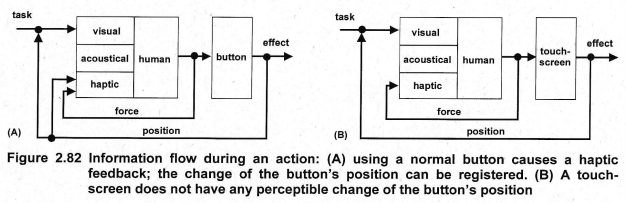
\includegraphics[width = 0.7\linewidth]{Figures/2_82.png}
	\end{figure}
	\item McGurk effect: If acoustic and visual stimuli are not correlated
\end{itemize}
\end{document}